\documentclass{article}
\usepackage[utf8]{inputenc}
\usepackage[parfill]{parskip}
\usepackage{hyperref}
\usepackage{amsmath}
\usepackage{amssymb}
\usepackage{amsfonts}
\usepackage{graphicx}
\usepackage{float}
\usepackage{listingsutf8}
\usepackage[dvipsnames]{xcolor}
\usepackage{listings}
\usepackage{fullpage}
\usepackage{caption}
\usepackage{tabto}


\title{Gestion de la memoire cache d'un serveur web}
\author{Nom : Grari \hspace{0.25cm} - \hspace{0.25cm} Prénom : Mohammed Achraf\hspace{0.25cm}  - \hspace{0.25cm} Matricule : 000509902\\\\Nom : Suau\hspace{0.25cm} -\hspace{0.25cm} Prenom : Thomas \hspace{0.25cm}-\hspace{0.25cm} Matricule : 000580972\\\\Nom : Massondi\hspace{0.25cm} -\hspace{0.25cm} Prenom : Williame \hspace{0.25cm}-\hspace{0.25cm} Matricule : 000568610\\\\Nom :Nguemayem Kaze\hspace{0.25cm} -\hspace{0.25cm} Prenom : Lydie Nadia \hspace{0.25cm}-\hspace{0.25cm} Matricule : 000509851 \\\\Nom : Meghadio Gonzeu\hspace{0.25cm} -\hspace{0.25cm} Prenom : Cedric Jordan  \hspace{0.25cm}-\hspace{0.25cm} Matricule : 000564114}
\date{15 mars 2023}
\begin{document}
\maketitle\hrule

  \begin{center}
  \vspace{1.5 cm}
    
\includegraphics[width=0.6\textwidth]{logo.png}
    \captionsetup{labelformat=empty}
    \label{fig:0}
  \end{center}
  
\newpage
\tableofcontents
\newpage

\section{Introduction}

%Les sites web prennent actuellement de plus en plus d'ampleurs et les gens étant plus connectés que jamais, le trafic peut rapidement devenir important et engendrer de nombreuses complications, comme le célèbre C10k problème pour les serveurs\footnote{Problème d'extension d'un serveur à partir de 10k utilisateurs  \href{https://en.wikipedia.org/wiki/C10k_problem#:~:text=The\%20C10k\%20problem\%20is\%20the,concurrently\%20handling\%20ten\%20thousand\%20connections}{Wikipedia c10k problem}.}.

Dans l'entreprise CoursParticuliers.com qui met en relation des enseignants avec des élèves, nous sommes administrateurs système. Le site web sert à informer sur ses services ainsi qu'un formulaire de contact. 
Récemment l'entreprise a comptabilisé un trafic important sur son site web et cela a engendré des ralentissements massifs ainsi que des bugs de fonctionnement pour l'utilisateur. 
Après avoir enquêté sur le problème nous en avons déduit qu'il s'agit d'une absence de gestion de la mémoire cache et d'un nombre de requêtes simultanées trop importantes. 
Ainsi nous pensons mettre en place une solution de caching afin de gérer le cache du site web. 

En informatique, un cache est une mémoire temporaire qui possède une date d'expiration. Le cache stocke des données intermédiaires entre le site (serveur) et l'utilisateur (client). La mise en cache nous permet de réutiliser efficacement des données précédemment récupérées ou traitées. Ainsi cela permet d'accélérer le flux sortant, autrement dit augmenter le nombre de demandes possibles sur le site. 
Cela permettrait donc d'augmenter grandement la vitesse et la réactivité du site web. 

Nous produisons ci-dessous notre rapport d'analyse des outils possibles ainsi que la solution choisie par l'équipe avec la justification de son bien fondé.

\subsection{Le contexte}

CoursParticuliers est une entreprise ayant beaucoup d'expérience avec l'enseignement qui s'est renommé CoursParticuliers.com afin de se positionner agressivement sur le web. Afin de développer ses outils numériques elle crée une division administration système pour gérer au mieux ses nouveaux services.
Le site web ne contenant actuellement qu'un formulaire de contact et des informations sur les enseignants subit déjà des ralentissements certainement relié à leur dernière campagne marketing. 
La campagne fut un franc succès et ramena plusieurs milliers d'utilisateurs sur le site.

Les examens approchent et CoursParticuliers.com ne veut pas rater cette opportunité. Néanmoins, les frais de maintenance et de gestion du site web sont exorbitants et doivent impérativement être réduits, afin de lancer une promotion unique offrant plusieurs heures de cours aux meilleurs étudiants qui permettrait à l'entreprise d'avoir une bonne réputation auprès de l'université et accroître son influence auprès des jeunes.
Une campagne de communication déjà bien rodée ; il faut trouver une solution efficace et la moins chère possible. 

L'open source est a favoriser tant que possible avec la possibilité d'avoir une branche entreprise disposant d'un service technique pour palier un problème urgent mettant en jeu la sécurité de l'entreprise ou le bon déroulement de la campagne marketing.

\subsection{Situation actuelle}

L'entreprise loue son serveur chez un géant du Web Hosting. Néanmoins, le paramétrage est très limité et ne nous permets pas d'implémenter notre code.
Nous n'avons en particulier aucune prise sur la mémoire cache au sein de l'hébergeur. 
L'accent a cette fois-ci été mis sur l'Open Source avec la location d'une petite configuration sur OVH, afin que notre équipe puisse développer de nouvelles solutions.
CoursParticuliers.com veut intégrer l'éthique et la gouvernance européenne dans ses valeurs c'est pourquoi ils sont allé chez OVH.

Le problème principal est de s'assurer de la disponibilité du site en période de très forte demandes. 
Aucun ralentissement ni bug ne doit apparaître pendant la campagne marketing. Il faut un système résilient et que l'utilisateur ait une expérience fluide pendant sa navigation.

Si la solution proposée est suffisamment efficace elle pourra donner lieu aux fondations du développement informatique de l'entreprise.
Nous souhaitons réellement participer au passage de l'entreprise sur le numérique et lui offrir les meilleurs outils pour la suite de sa croissance.
Un nouveau type de cours particuliers peut voir le jour et aura besoin d'un système configurable, simple et disponible partout rapidement.

Cela serait un plus suite à notre recherche mais notre priorité reste la mémoire cache du site pour sa fluidité, non négociable en cette période.

Nous devons donc trouver un système de gestion de la mémoire cache qui se connectera aisément au serveur sur lequel on pourra si besoin prendre la main.

% Apache car on n'a pas fait de recherches dessus mais faut l'aborder car NGINX est mieux. Au moins ici ça nous évite de le définir tout ça mais on peut l'utiliser pour les comparaisons.
Nous avons lancer Apache sur l'instance louée par l'entreprise afin de mener notre recherche sur les logiciels de gestion du cache.


\section{Avantages de la mise en cache}

\subsection{Amélioration des performances de l'application}

Comme le cache est beaucoup plus véloce que le disque dur (magnétique ou SSD), la lecture des données à partir du cache en mémoire est extrêmement rapide (infra-milliseconde). Cet accès aux données significativement plus rapide améliore les performances globales de l'application.


\subsection{Réduction des coûts de base de données}

Une seule instance de cache peut fournir des centaines de milliers d'IOPS (opérations d'entrée/sortie par seconde), remplaçant potentiellement un certain nombre d'instances de base de données, ce qui permet de réduire le coût total. Cela est particulièrement important si la base de données primaire facture au débit. Dans ce cas, les économies pourraient être considérables.

\subsection {Réduction de la charge sur le backend}

Le backend est responsable de tout ce qui se passe en coulisses pour faire fonctionner un site web. En redirigeant d'importantes parties de la charge de lecture de la base de données vers la couche en mémoire, la mise en cache peut réduire la charge sur notre base de données et la protéger contre les baisses de performances sous charge, ou même contre le plantage pendant les périodes de pics.

\subsection {Performances prévisibles}

Un défi courant dans les applications modernes est la gestion des périodes de pics dans l'utilisation des applications. Parmi les exemples, on trouve des applications sociales pendant le Super Bowl ou le jour des élections, les sites Web d'e-commerce pendant le Black Friday, etc. Une augmentation de la charge sur la base de données génère des latences plus élevées pour obtenir les données, ce qui rend les performances d'application imprévisibles. En utilisant un débit élevé de cache en mémoire, ce problème peut être atténué.

\subsection{Performances prévisibles : Élimination des hotspots de base de données}

Dans la plupart des applications, il est probable qu'un petit sous-ensemble de données, tel qu'un profil de célébrité ou un produit populaire, soit visité plus fréquemment que d'autres. Cela peut provoquer des points chauds dans notre base de données et nécessiter un surprovisionnement de ressources de base de données en fonction des exigences en matière de débit pour les données les plus fréquemment utilisées. Le stockage de clés courantes dans un cache en mémoire diminue le besoin de surprovisionner tout en fournissant des performances élevées et prévisibles pour les données les plus fréquemment consultées.


\subsection{Augmentation du débit de lecture (Entrées/Sorties par seconde)}

En plus d'une latence plus faible, les systèmes en mémoire proposent également des taux de demande (IOPS) beaucoup plus élevés par rapport à une base de données basée sur disques comparable. Une instance unique utilisée comme cache distribué peut servir des centaines de milliers de requêtes par seconde.





\section{Analyse des outils}

\subsection{Varnish}

Varnish agit comme un cache de reverse proxy HTTP, et parfois il est décrit comme un accélérateur front-end (la partie visible d'un site web ).

Un {\it reverse proxy} signifie qu'il va se placer comme intermédiaire entre l'utilisateur et le serveur. D'un point de vue technique, l'utilisateur ne va pas se connecter directement au serveur mais à Varnish qui va lui-même se connecter au serveur pour obtenir les informations demandées par l'utilisateur.
\begin{figure}[h!]
    \centering
    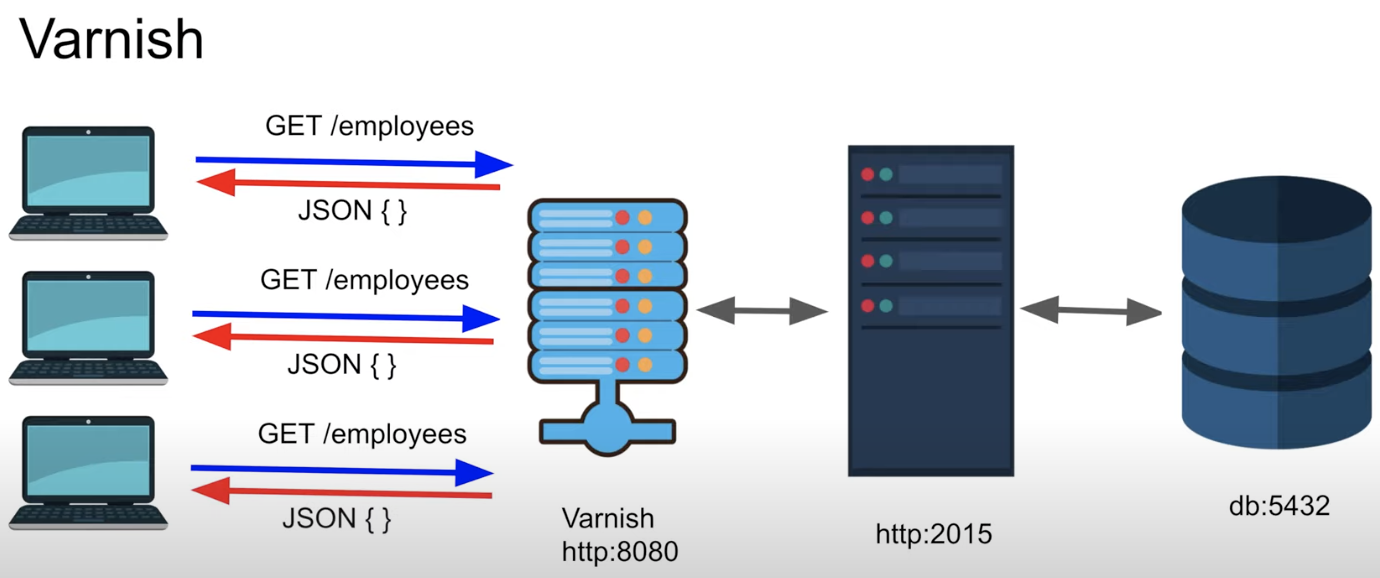
\includegraphics[scale=0.4]{Varnish_schema.png}
    \caption{Fonctionnement de Varnish}
    \label{fig:varnish-schema}
\end{figure}


\hspace{0.1cm}

Dans le schéma ci-dessus, l'utilisateur demande à accéder à la section \texttt{employees}. Il fait donc la requête auprès de Varnish qui lui-même demande une fois au serveur puis il répond (\texttt{JSON} signifie simplement le format de réponse).
Après avoir fait cette opération, il ne la fait plus et envoie le résultat précédent aux suivants. Le gain de temps, d'énergie et d'efficacité est dès lors évident.

Ce n’est pas une solution indépendante car elle a besoin d’un serveur web dédié sur lequel se baser comme Apache ou Nodejs.
Varnish est utilisable en ligne de commande, ce qui est pour nous un bon point afin d'avoir une large marge de manœuvre.

On peut utiliser Varnish pour mettre en cache beaucoup de types de contenus : c’est une solution efficace pour améliorer non seulement la vitesse de notre site web, mais également nos performances serveur.

\hspace{0.1cm}

{\bf Avantages} :\\
\begin{itemize}
    \item Solution spécialisée dans le caching et permettant une des plus grandes personnalisation du cache sur le marché. Cela peut permettre d'adopter des stratégies de cache très développées.
    \item Open-Source et orienté business avec une offre pro très développée et un service réactif.
    \item La communauté de Varnish est développée ce qui doit nous permettre d'avoir un accompagnement assez précis tout au long de notre implémentation et du suivi de la solution.
    \item Les données seront stockées sur le disque dur du serveur puis mise en cache par Varnish sur son instance. 
    \item Utilisation en ligne de commande.
    \item On peut utiliser des outils simples pour tester nos premières configuration (docker via un conteneur varnish dédié). 
    \item Le livre {\it Varnish 6 by Examples} qui accompagne l'administrateur tout au long du parcours Varnish.

\end{itemize}

\hspace{0.1cm}

{\bf Inconvénients} :\\
\begin{itemize}
    \item Pas de gestion du serveur. Se connecte aisément à Apache mais représente un outil suppélmentaire.
    \item Davantage de complexité, notamment avec la configuration qui nécessite la manipulation du langage Varnish Configuration Language (VCL).
    \item  Aucune prise en charge native des connexions sécurisées (TLS/SSH ou HTTPS). Il faut utiliser des intermédiaires (comme Caddy pour ajouter les connexions sécurisées type HTTPS) ce qui peut compléxifier le serveur.
    \item Adapté uniquement aux systèmes d’exploitation sous Unix.
    \item Ne répond pas à la perspective d'évolutivité de CoursParticuliers.com.
 
\end{itemize}


\subsection{NGINX}

NGINX est un serveur web open source populaire, connu pour sa haute performance, sa fiabilité et sa souplesse. Initialement développé pour les sites web à forte demande de trafic, il est aujourd'hui utilisé pour une variété de tâches, notamment comme serveur web.\\

NGINX peut gérer des milliers de connexions simultanées avec une utilisation minimale des ressources système. Il est également capable de servir des contenus statiques de manière très efficace et de répartir la charge entre plusieurs serveurs.\\

NGINX est connu pour sa sécurité, sa flexibilité et sa facilité d'utilisation. Il dispose également d'une large communauté de développeurs qui travaillent continuellement à son amélioration et à son développement, ce qui en fait un choix populaire pour les entreprises et les organisations de toutes tailles.
\begin{figure}[h]
    \centering
    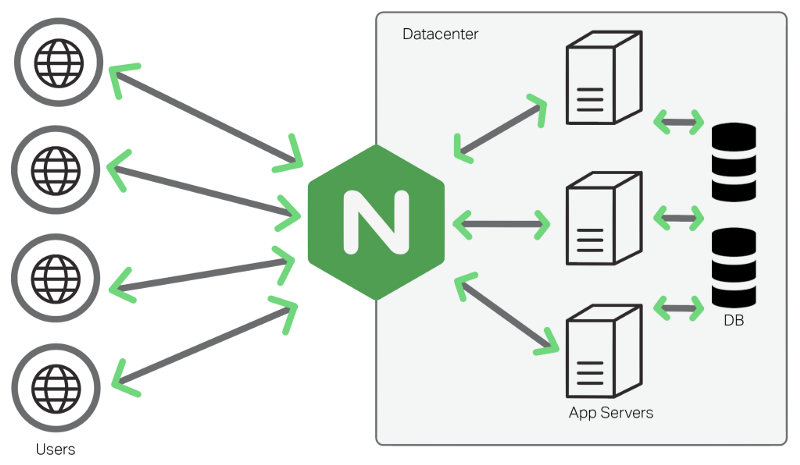
\includegraphics[scale=0.4]{NGINX.png}
    \caption{Fonctionnement de NGINX}
    \label{fig:NGINX-schema}
\end{figure}

\hspace{0.1cm}

{\bf Avantages :}\\

 NGINX est un outil qui permet de mettre un site web en ligne sur internet. Il assure plusieurs tâches importantes pour que le site fonctionne bien et soit sécurisé.\\

\begin{itemize}
    \item En tant que serveur web, NGINX sert les pages web et permet aux utilisateurs d'y accéder depuis leur navigateur internet.\\

    \item En tant que répartisseur de charge, NGINX s'assure que le site web est disponible pour les utilisateurs même si beaucoup de personnes essaient de l'utiliser en même temps. C'est un peu comme avoir plusieurs portes d'entrée pour une boutique très populaire pour éviter les bousculades et les files d'attente.\\

    \item En tant que reverse proxy, NGINX protège le site web des attaques informatiques en bloquant les personnes mal intentionnées. C'est un peu comme avoir un garde du corps pour le site web qui empêche les intrus de causer des dégâts.\\

    \item En tant que proxy de cache, NGINX stocke temporairement certaines informations pour que le site web soit plus rapide et plus efficace. C'est comme avoir un cerveau qui se souvient de ce que les utilisateurs ont déjà vu pour leur montrer plus rapidement s'ils reviennent sur le site.\\
\end{itemize}

En somme, NGINX est un outil très utile pour mettre un site web en ligne, le protéger des attaques et s'assurer qu'il fonctionne bien même avec beaucoup de visiteurs.\\

\hspace{0.1cm}

{\bf Inconvénients :}\\
\begin{itemize}
    \item Pas d'interface graphique : NGINX est principalement utilisé en ligne de commande, ce qui peut être difficile pour les administrateurs qui préfèrent une interface graphique conviviale.
    Cependant, il existe des outils tiers qui peuvent aider à simplifier la configuration de NGINX en utilisant une interface graphique. Par exemple, certains panneaux de contrôle de serveur web tels que cPanel, Plesk et ISPConfig prennent en charge la configuration de NGINX via une interface graphique. Il existe également des outils open source tels que Webmin et Ajenti qui proposent une interface web pour la gestion de serveurs, y compris NGINX. Cependant, il est important de noter que ces outils tiers peuvent ne pas offrir toutes les fonctionnalités de NGINX, ou peuvent être moins flexibles que la configuration manuelle en ligne de commande. De plus, la configuration manuelle peut offrir un meilleur contrôle sur les performances et la sécurité du serveur web.\\

    \item Pas de support officiel : il est vrai que pour les utilisateurs de NGINX open source (c'est-à-dire ceux qui n'utilisent pas la version commerciale de NGINX proposée par NGINX, Inc.), il n'y a pas de support officiel directement fourni par NGINX, Inc. Cependant, il existe de nombreuses ressources communautaires disponibles, notamment des forums, des listes de diffusion et des documentations en ligne, qui peuvent aider les utilisateurs à résoudre les problèmes et à obtenir de l'aide en cas de besoin.\\ 
\end{itemize}

\hspace{0.1cm}

{\bf Optimiser la mise en cache des cookies :}\\

La mise en cache des cookies est une technique pour améliorer les performances des sites web. Les cookies sont des petits fichiers qui contiennent des informations sur l'utilisateur et sont stockés sur l'ordinateur de l'utilisateur. Certains cookies ne changent pas souvent, tandis que d'autres changent fréquemment.

Pour les cookies statiques qui sont identiques pour tous les utilisateurs, il est possible de les mettre en cache pour les livrer plus rapidement aux utilisateurs. Cela permet d'éviter une surcharge inutile du serveur et de réduire le nombre de requêtes envoyées au serveur, ce qui améliore les performances.

Pour les cookies dynamiques qui changent fréquemment et qui sont spécifiques à chaque utilisateur, il est possible de les mettre en cache en fonction de leur durée de vie. Cela permet de réduire la latence lors du chargement des pages pour les utilisateurs, car les cookies sont livrés plus rapidement.

Enfin, il est possible de compresser les cookies avant de les envoyer aux utilisateurs. Cela permet de réduire la taille des cookies et d'améliorer les performances du site web en réduisant la quantité de données à transférer sur le réseau.


\subsection{Squid Cache}

Squid Cache est un serveur proxy Web open source. Il est utilisé pour améliorer les performances du réseau et la sécurité du système d'information. Squid Cache met en cache des pages Web, des images et d'autres contenus.
Des demandes fréquentes sont maintenues, ce qui permet d'accélérer leur récupération (gestion de la pré-génération de contenu). En plus de la mise en cache des pages Web, Squid Cache peut également être utilisé pour filtrer le trafic réseau selon certaines règles. Cela peut contribuer à accroître la sécurité de nos systèmes informatiques.
Squid Cache est open source et ne bénéficie pas d'un service client disponible pour les entreprises.

\hspace{0.1cm}

{\bf Avantages} :\\
\begin{itemize}
    \item Fonctionnalités de sécurité : Squid Cache peut également être utilisé pour filtrer le trafic web en fonction de certaines règles, ce qui peut contribuer à améliorer la sécurité des systèmes d'information.\\
    
    \item Open Source : Répond donc aux éxigences de la hiérarchie.\\
    
    \item Large communauté : Squid Cache a une large communauté d'utilisateurs et de contributeurs, ce qui signifie qu'il existe de nombreuses ressources disponibles en ligne pour aider les utilisateurs à résoudre les problèmes.\\
\end{itemize}

\hspace{0.1cm}

{\bf Inconvénients} : \\
\begin{itemize}
    \item Configuration complexe : Squid Cache peut être difficile à configurer.\\
    
    \item Besoin de beaucoup de ressources matérielles : Squid Cache nécessite des ressources matérielles pour fonctionner correctement, notamment de la mémoire vive et de l'espace de stockage pour le cache.\\    
\end{itemize}

En résumé, Squid Cache est un serveur proxy web puissant et polyvalent, qui peut être utilisé pour améliorer les performances web et la sécurité des systèmes d'information. Toutefois, sa configuration peut être complexe et il nécessite d'importan ressources matérielles pour fonctionner correctement.

\section{La solution choisie}

L'équipe a fait le choix de {\bf NGINX}. Cela pour plusieurs raisons que l'on va détailler ci-dessous. L'implémentation devrait être achevée pour le 7 mai 2023 avec un rapport détaillant cette implémentation pour le service technique.\\ 
% Mini phrase de conclusion puis go sur la partie Pourquoi NGINX
\subsection{Role de NGNIX}

L'utilisation la plus fréquente de Nginx est de le configurer comme un serveur Web classique. Il remplacerai Apache dans notre configuration actuelle et nous permettrait de gérer le cache directement à l'intérieur. 


\subsection{Pourquoi NGINX ?}

Nginx apporte à la fois la manipulation en ligne de commande, avec un téléchargement simple et donc mobile sur l'ensemble du parc des machines de l'entreprise.
A la fois simple à prendre en main et complet, il peut parfaitement convenir à nos besoins de gestion globale du serveur. 

En particulier, Nginx répond également au besoin de modularité future voulue par le conseil d'administration de CoursParticuliers.com.

 \subsubsection{Avantages de NGNIX}

Nginx a été conçu conçu pour répondre au problème C10K\footnote{Pour plus de détail on pourra consulter :  \href{https://en.wikipedia.org/wiki/C10k_problem#:~:text=The\%20C10k\%20problem\%20is\%20the,concurrently\%20handling\%20ten\%20thousand\%20connections}{Wikipedia c10k problem}.}où le but est d'être capable de répondre à plus de 10 000 reqêtes simultanées. 

Nginx sera modulable selon nos besoins et offrira une évolutivité pour la suite des développements de l'entreprise.


\subsection{Configuration nécessaire}

Nginx requiert une instance accessible 7/7j 24/24h, mais ne requiert pas de stockage ou de configuration spécifique pour marcher. 
Nginx permettra donc à CoursParticuliers.com de nettes économies sur les abonnements serveurs.

\subsection{Planning d'implémentation}


Du 10/04 au 16/04 : Implémentation du serveur et de tous l’aspect technique nous permettant d’implémenter notre solution (avec prise en main de Nginx par l'équipe). 

Du 17/04 au 23/04 : Implémentation de la solution avec toute l’équipe. 

Du 24/04 au 31/04 : Rédaction du rapport technique d'utilisation et de configuration destiné aux développeurs. 


\end{document}

